%% ----------------------------------------------------------------
%% ObjectDetection.tex
%% ---------------------------------------------------------------- 
\chapter{Recent Work in Object Detection} \label{Chapter:ObjectDetection}

Object detection is the natural extension of the image classification problem. In image classification, for each sample, there is a single output denoting the class of the sample. In mathematical notation for each sample $\textbf{X}$, $\phi(\textbf{X})$, gives as output an $N-$vector $\textbf{P}_x=(p_1,p_2,...,p_N)$\footnote{$\sum^N_i p_i=1$}, where each element indicates the probability of the sample belonging to the class $n_i \in N$ and $\phi$ denotes the model. Object detection pushes this task a bit further by classifying and localising an instance in the image, instead of merely making a prediction. Therefore, for each sample query, the output is represented by the predicted class and a set of coordinates that define a bounding box around the object; there could be more than one predictions for a single image. Despite that traditional object detection generates a rectangular bounding box around the predicted objects, the vision community developed object detection into more advanced tasks, such as image and instance segmentation. In image segmentation, the model is called to classify images pixel-wise where each pixel represents a class, while in instance segmentation the model segments the observed classes into objects and background (\fref{ch2:fig1}). While object detection was an active field many years before deep learning, the most notable and robust algorithms have been developed practising deep learning techniques. In general, deep learning-based object detectors are divided into \textbf{\textit{double-stage detectors}} and \textbf{\textit{single-stage detectors}}. An overview of these methods is given in the next sections, along with the most significant models. 

\begin{figure}[!htb]
  \centering
  \subfigure[Classification.]{
    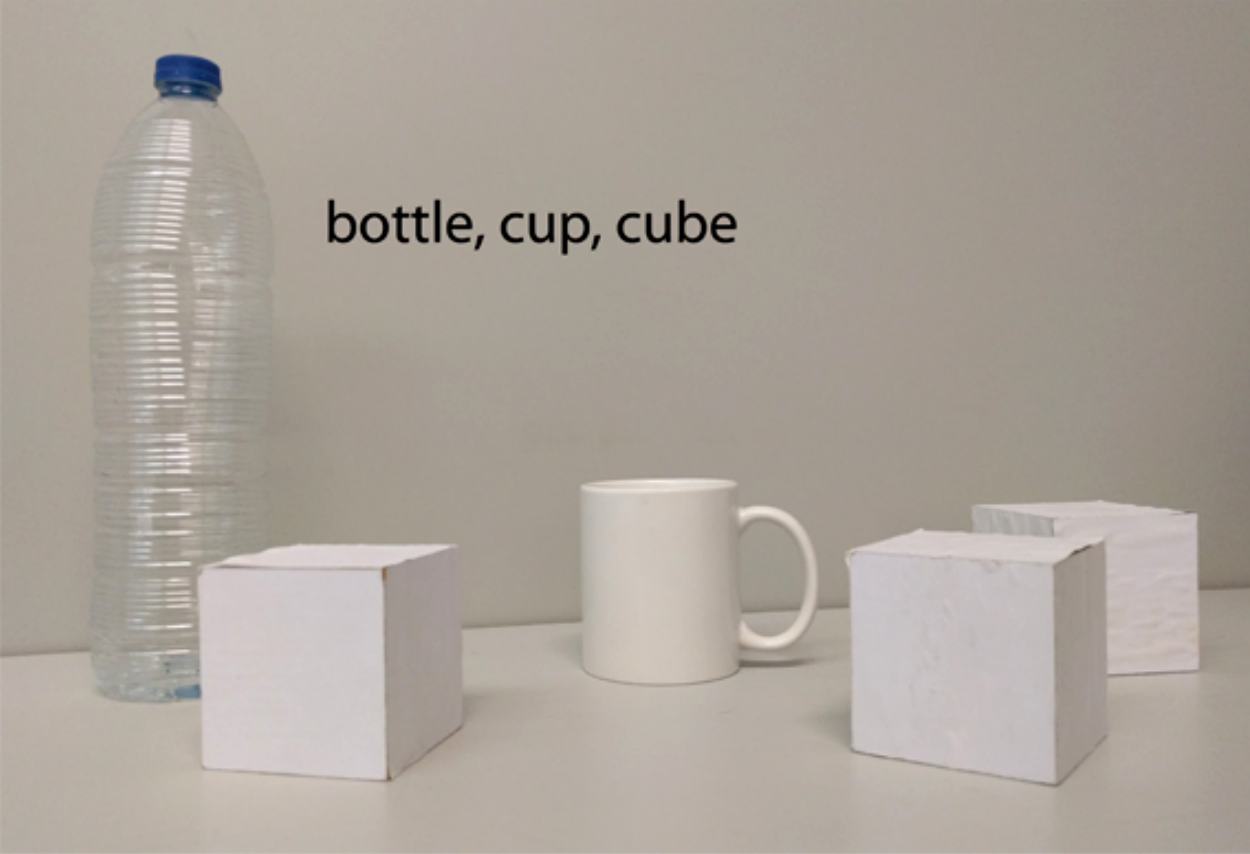
\includegraphics[width=4cm]{figures/ch2/fig1_1.png}
    \label{ch2:fig1_1}
  }
  \subfigure[Detection (classification + localisation).]{
    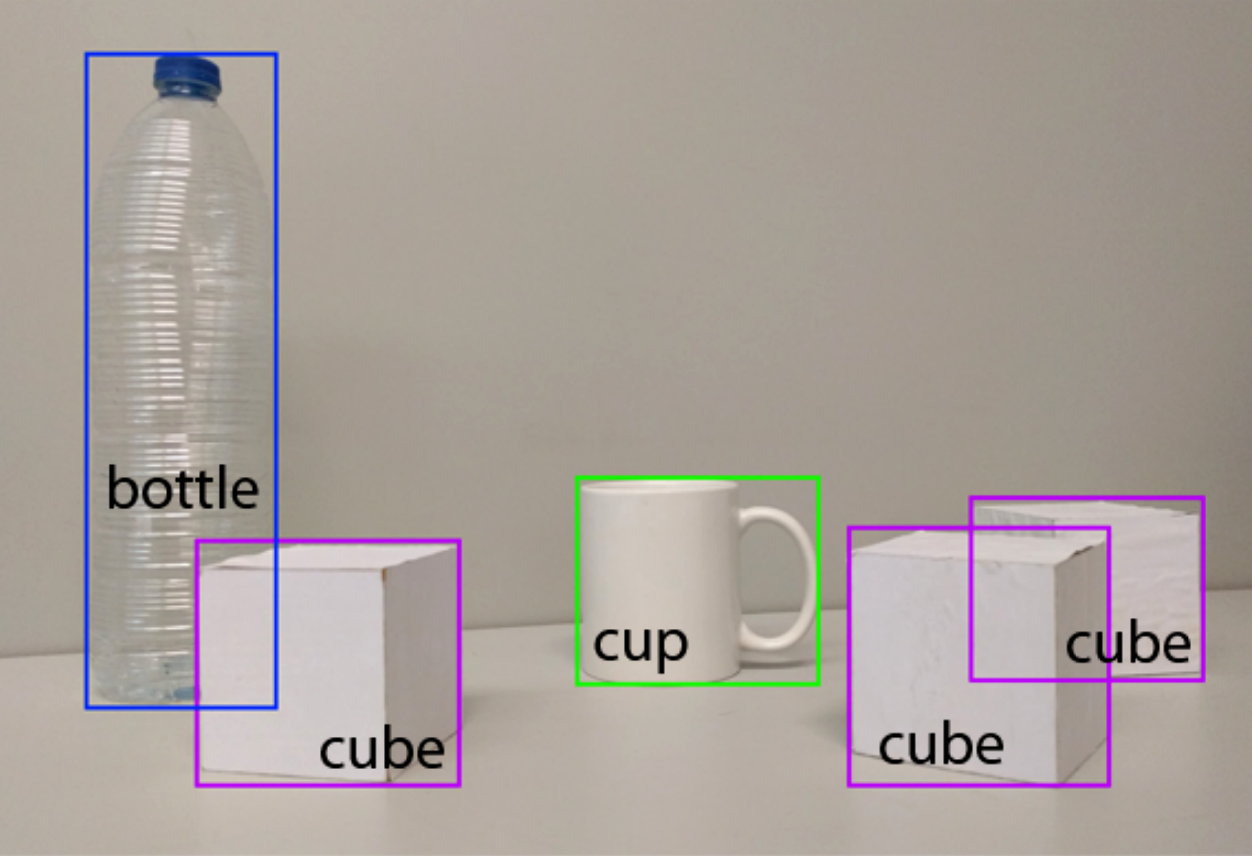
\includegraphics[width=4cm]{figures/ch2/fig1_2.png}
    \label{ch2:fig1_2}
  }
  
    \subfigure[Image segmentation.]{
    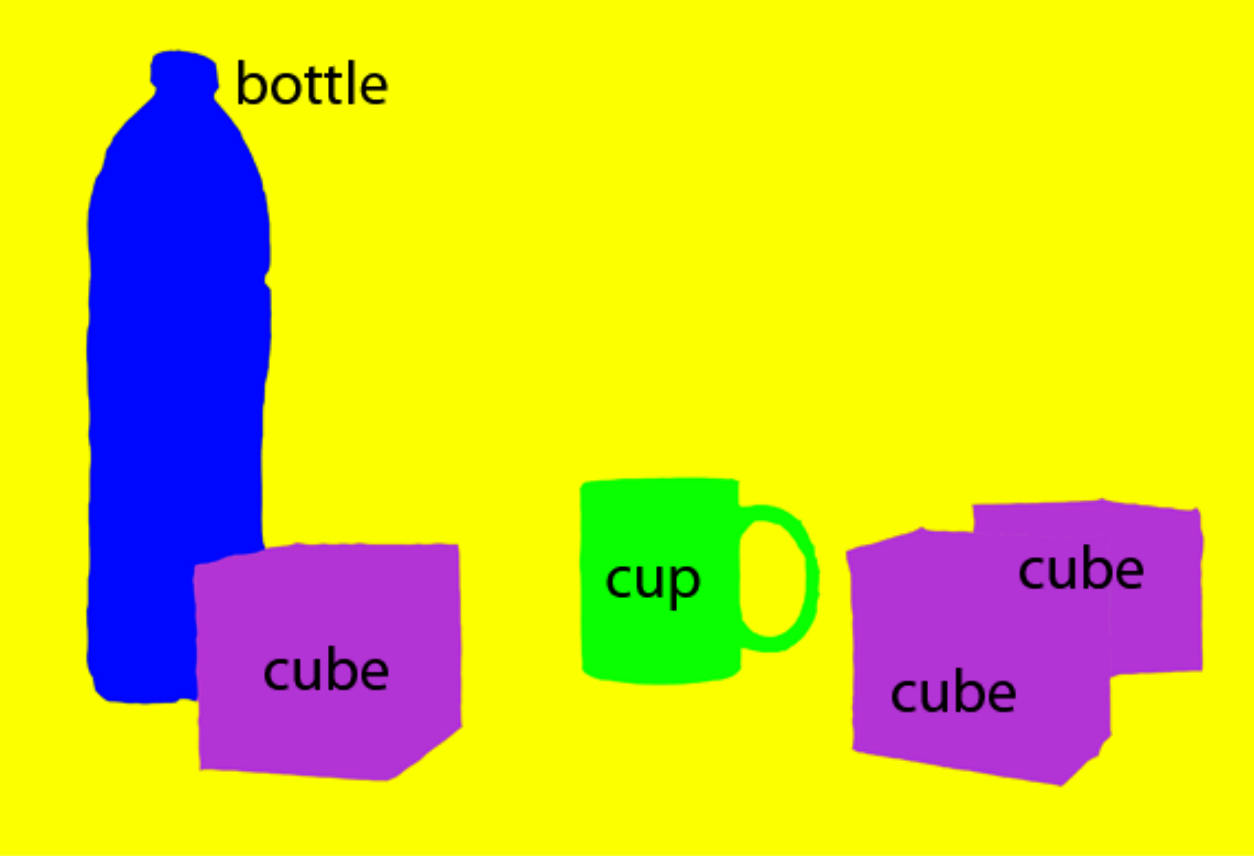
\includegraphics[width=4cm]{figures/ch2/fig1_3.png}
    \label{ch2:fig1_3}
  }
    \subfigure[Instance segmentation.]{
    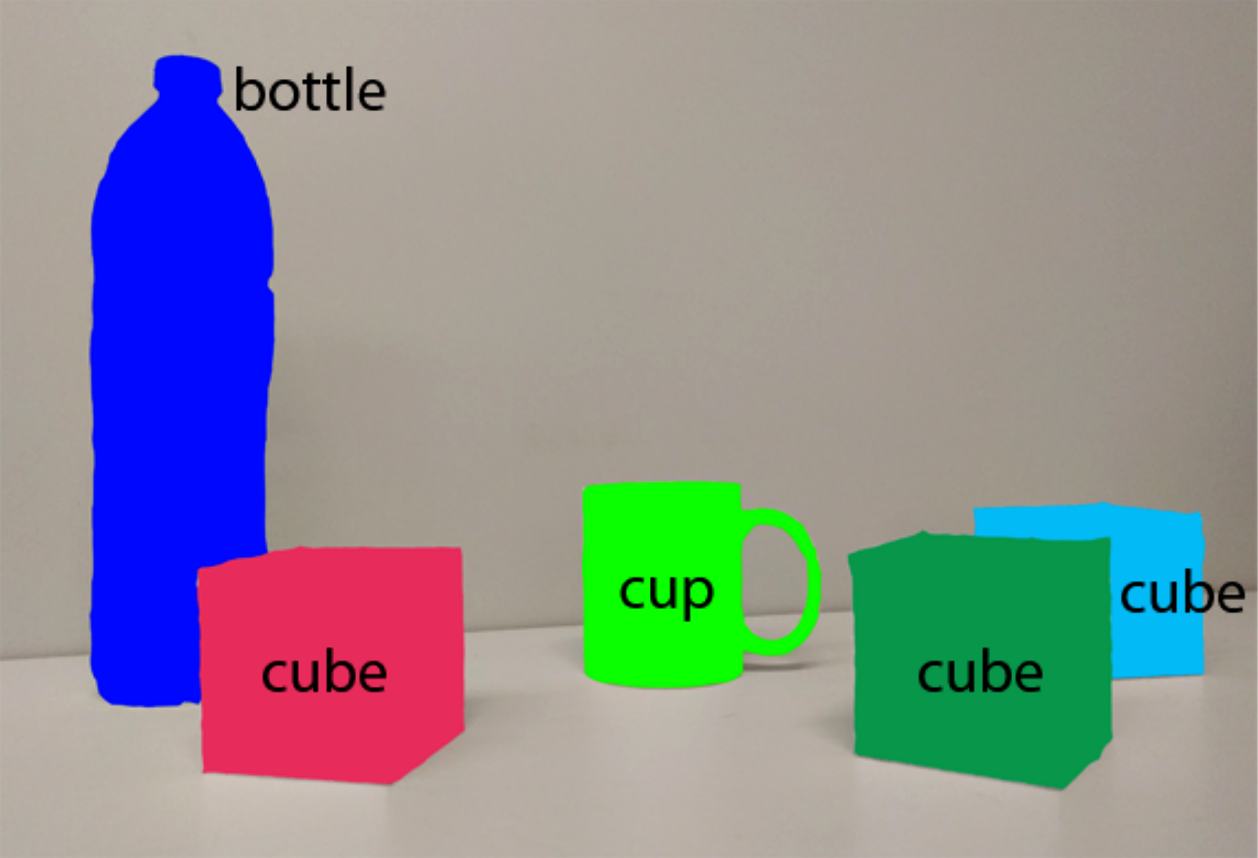
\includegraphics[width=4cm]{figures/ch2/fig1_4.png}
    \label{ch2:fig1_4}
  }
  \caption{Image analysis tasks (Reproduced from \cite{garcia1704review}), where the model: (a) Produces an $N-$vector with the probability of each class being present in the image. (b) Produces a set of coordinates for every predicted image. (c) Classifies the image pixel-wise in classes. (d) Classifies pixel-wise only the relevant instances ignoring background.}
  \label{ch2:fig1}
\end{figure}

\section{Double-Stage Detectors}

The detection process in double-stage or \textbf{\textit{region proposal based detectors}} can be split into two parts. The first part generates class-agnostic regions of interest (RoI) defined by a bounding box, and the second part predicts the class of each proposed RoI and refines the bounding box around them. The most popular method in double stage detectors is called "Regions with CNN features" and includes R-CNN (\cite{girshick2014rich}), and its successors Fast R-CNN (\cite{girshick2015fast}) and Faster R-CNN (\cite{ren2015faster}).

\subsection{R-CNN}
R-CNN was the first method that outperformed the previous state-of-the-art CNN method, OverFeat (\cite{sermanet2013overfeat}), increasing accuracy by a notable margin. Specifically, R-CNN achieved a mean average precision (mAP) of 31.4\% on the ILSVRC2013 (\cite{deng2009imagenet}) dataset, over OverFeat which had the previous best results (24.3\%).

R-CNN consists of three parts. The first part generates 2000 class-agnostic regions of interest using selective search (\cite{uijlings2013selective}), with most of them being negative examples. Each proposed region of interest acts as a potential detection defined by its bounding box. Then, these proposals are warped into a fixed size defined by the architecture's input size. 
The second part is a CNN, pre-trained on the ImageNet dataset (fine-tuned on the new data) working as a feature extractor from its last fully connected layer. In the last step, the 4096-dimensional extracted features from each RoI, are classified by $N$ class-specific, plus one (background), SVMs. Finally, for each positive prediction, class-specific box regressors regress the bounding box offsets resulting in a refined bounding box.

\begin{figure}[!htb]
  \centering
  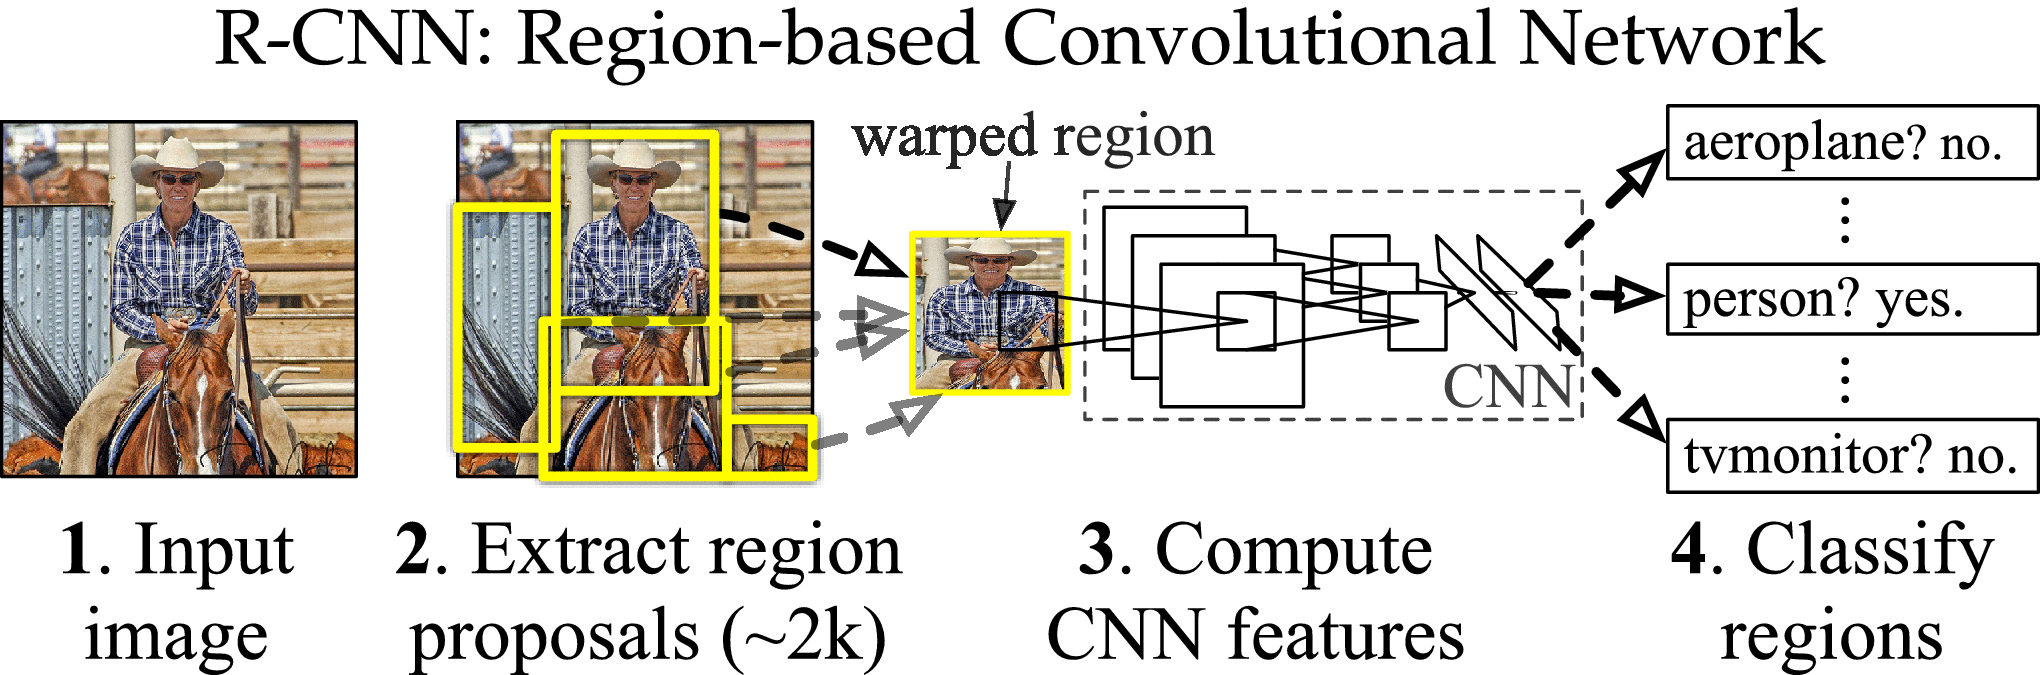
\includegraphics[width=12cm]{figures/ch2/fig2.png}
  \caption{R-CNN pipeline as presented in \cite{girshick2014rich}.}
  \label{ch2:fig2}
\end{figure}

Despite that R-CNN increased the performance margin strikingly, it has the following notable drawbacks:

\begin{itemize}
  \item The selective search is a heuristic-based algorithm; thus, it is unable to learn anything during the training procedure. 
  \item Training time needs a vast amount of time and disk space, considering that for each image, 2000 proposals have to be fed to the network. Since training it is a multi-stage pipeline, extracted features have to be cached on disk before passed to the SVMs and box regressors. Notice that since the majority of samples are negatives, the authors adopted hard negative mining forcing the model to focus on hard examples (\cite{felzenszwalb2009object}) in order to accelerate convergence.
  \item It is not suitable for real-time applications as it has a GPU test rate of  47 seconds/images when OverFeat is 9x times faster (\cite{girshick2015fast}). 
\end{itemize}

\subsection{Fast R-CNN}
Fast R-CNN was introduced as the improved version of R-CNN, where the multi-stage network was replaced by a single-stage pipeline able to be trained in one stage.

\begin{figure}[!htb]
  \centering
  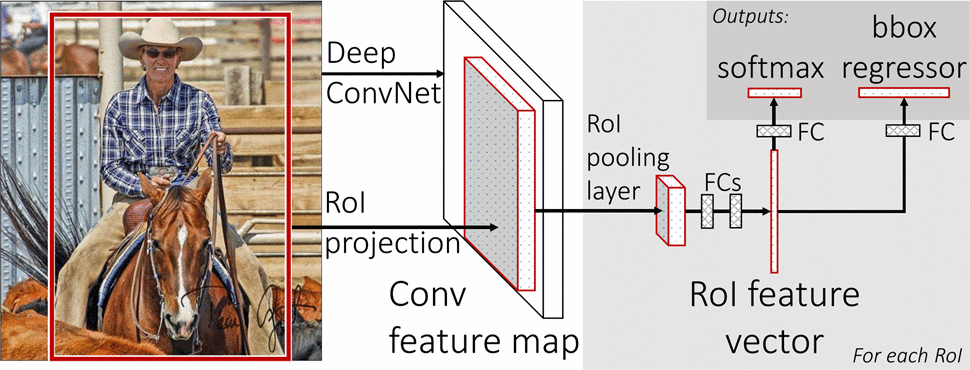
\includegraphics[width=12cm, height=3cm]{figures/ch2/fig3.png}
  \caption{Fast R-CNN pipeline as presented in \cite{girshick2015fast}.}
  \label{ch2:fig3}
\end{figure}

To achieve this, Fast R-CNN adopted a method from SPP-net (\cite{he2015spatial}) called RoI pooling. R-CNN was handling proposals by warping them into a fixed size and feeding them into the network one by one. On the contrary, SPP-net and Fast R-CNN compute varying sized feature maps of the entire image instead of warped region proposals. Each feature map contains RoI information in a four-tuple $(r,c,h,w)$, where $r, c:$ top-left corner and $w, h:$ width and height. \fref{ch2:fig4} presents how the RoI pooling layer extracts fixed-length feature vectors from varying sized maps.

Moreover, the SVMs and the box regressors have been replaced by a joint sibling layer consisting of a softmax layer and a box regressor. Softmax produces a class probability over K + 1 classes (including background), while the regressor predicts the offsets for the refined bounding boxes. \fref{ch2:fig3} illustrates an overview of the model. 

\begin{figure}[!htb]
  \centering
  \subfigure[Feature map with 2 RoIs.]{
    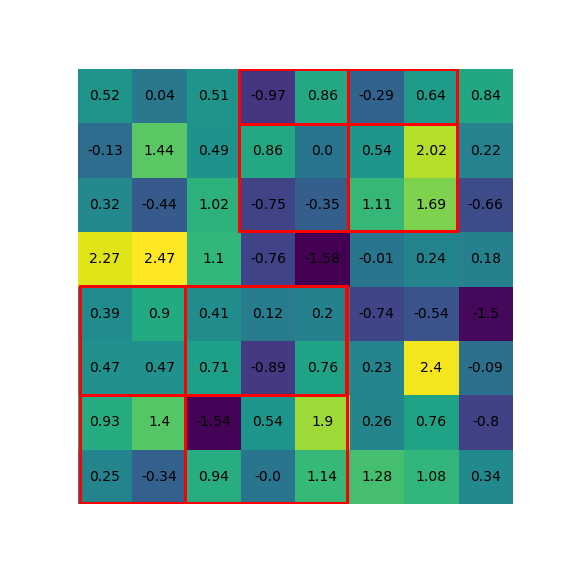
\includegraphics[width=6cm]{figures/ch2/fig4_1.png}
    \label{ch2:fig4_1}
  }
  \subfigure[Fixed sized RoIs after RoI pooling.]{
    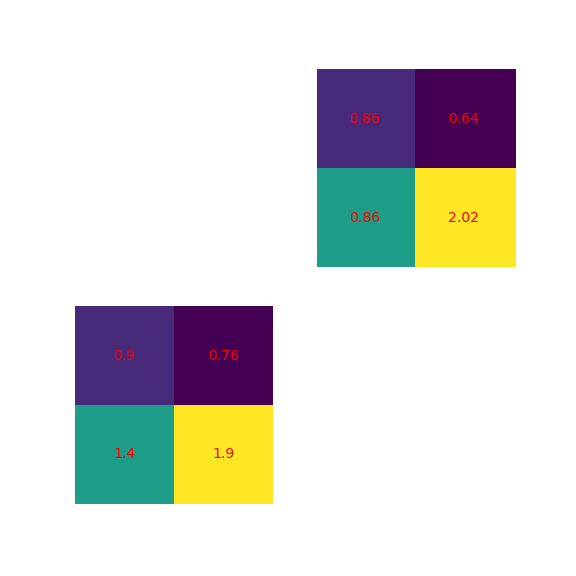
\includegraphics[width=6cm]{figures/ch2/fig4_2.png}
    \label{ch2:fig4_2}
  }
  \caption{RoI pooling layer. To extract fixed-length feature maps, different sized proposed RoIs are divided into a fixed number of bins appropriately.}
  \label{ch2:fig4}
\end{figure}

By feeding the entire image into the network instead of $\sim$2k proposals one by one, the network avoids redundant computations since many proposals are overlapping each other, hence it is more efficient than its predecessor both in terms of time and memory. Specifically, it is 10x faster than R-CNN in training time and 213x in testing. Furthermore, a joint loss $\mathcal{L}=\mathcal{L}_{cls}+\mathcal{L}_{reg}$ from the softmax and the regression layers optimises the network.

\subsection{Faster R-CNN}
After the integration of the joint sibling layer to the main network, Fast R-CNN was the state-of-the-art object detector, based almost entirely on convolutional neural networks. Its primary disadvantage was that the region proposal method, selective search, was not a learning method but a heuristic approach. Shortly, this was fixed by the introduction of Faster R-CNN (\cite{ren2015faster}) which entirely replaced selective search with a trainable region proposal network (RPN). RPN is a CNN where the network's output is attached to a class predictor and a box regressor. The class predictor has only two classes (object, not object); thus, the network is trained to propose regions of interest by their "\textit{objectness}". The rest of the network adopts the pipeline of the Fast R-CNN. Faster R-CNN is classified as a double-stage detector even if the region proposal method is not decoupled, anymore, from the main pipeline, due to its 4-step alternate training. Its training steps are synopsised below:
 
\begin{enumerate}
  \item RPN is initialised on the ImageNet weights and gets fine-tuned for the region proposal task.
  \item The detector (Fast R-CNN) is initialised on the ImageNet weights and gets fine-tuned for the detection task, with the proposed regions of interest from the RPN (the two models do not share any convolutional layers yet).
  \item The detector is used to initialise the RPN training, by keeping the weights coming from shared layers constant and updates only the weights coming from the unique layers. At this point, the two models share convolutional layers.
  \item Finally, the detector's unique layers are fine-tuned, keeping constant the weights from the common convolutional layers.
\end{enumerate}

Faster R-CNN's greatest success is that it consists of a single-stage end-to-end trainable network, entirely based on CNNs with an inference time of 5 FPS.


\section{Single-Stage Detectors}
The downside of double-stage detection is that training time is split into two separate parts, the region proposal and the detection part, hindering real-time detection. Single-stage detectors or \textbf{\textit{regression/classification based detectors}} have the advantage of being very fast. The main reason is that instead of making class predictions and refining bounding boxes on already proposed regions, they apply global rules in every pixel inferring relevant detections without intermediate mechanisms. SSD (\cite{liu2016ssd}), YOLO (\cite{redmon2016you}) and RetinaNet (\cite{lin2017focal}) are the most notable frameworks in this category.
 
 \subsection{YOLO}
 YOLO, developed by \cite{redmon2016you} (followed by the improved versions of YOLOv2 (\cite{redmon2017yolo9000}) and YOLOv3 (\cite{redmon2018yolov3})) is a model known for its rapid inference 
 rates ranging between 20-220FPS (depending on the backbone implementation) based entirely on Darknet; a network developed by Redmon.
 
The idea behind YOLO is to obtain detections from each pixel individually instead of relying on region proposal methods. An image $W\times H$ is fed into the backbone network activating an output map of size $S\times S$, right after the last convolutional layer. Each pixel (or grid-cell) in the given feature map (or grid) represents an area in the original image of $\frac{W}{S} \times \frac{H}{S}$ pixels and is responsible for detecting an object that has its centre on that cell. For example, if an object lies in the bottom right corner of the original image, the pixel $(S,0)$ on the feature map is responsible for its detection. If an object lies in the middle of the image, the pixel $(\frac{S}{2},\frac{S}{2})$ is responsible for its detection. 
 
\begin{figure}[!htb]
  \centering
  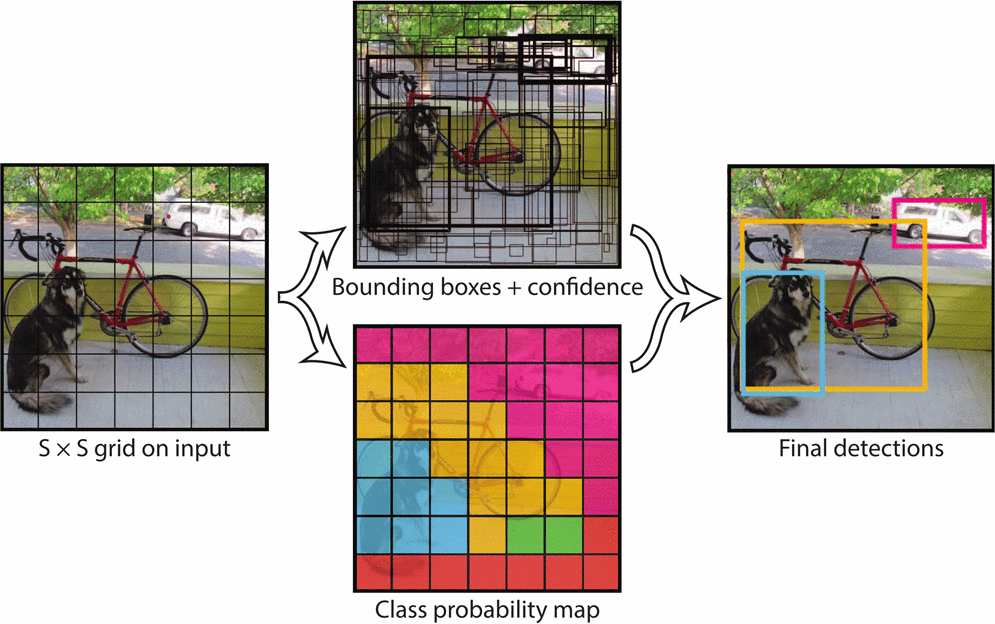
\includegraphics[width=12cm]{figures/ch2/fig5.png}
  \caption{A representation of how grid cells detect objects in the YOLO model: Each cell is responsible for detecting the object in its centre. The 8 blue pixels in the image produce a $p(\text{dog}|obj)$. If their boxes overlap each other (which can be seen from the top image), the one with the highest $p(\text{dog}|obj)$ is proposed and the others are suppressed. Reproduced from \cite{redmon2016you}.}
  \label{ch2:fig5}
\end{figure} 
 
The actual volume of the feature map sized $S\times S$, is an $S\times S \times (B\times5+C)$ tensor, where 5 in the parentheses implies the four coordinates of the B predictions and an objectness score $p(obj)$ which is expressed by the overlap of the box with the ground truth. Also, for each grid cell, a C-sized vector is predicted, indicating $p(c_i|obj)$. Each cell makes B predictions but only of one class, defined by the probability $p(c_i|obj)$. 

YOLO is limited in making B predictions in each grid cell but only of one class. This limitation makes difficult the detection of small objects in groups. The next versions of YOLO, are capable of making predictions in intermediate layers (from different sized feature maps) enabling detection in various scales and sizes. 
 
\subsection{SSD}
Single Shot Detector (or SSD) was published right after YOLO by \cite{liu2016ssd} and aimed to solve YOLO problems. SSD follows an architecture based on VGG16 (as Faster R-CNN) and operates similar to YOLO. The first version of Redmon's detector had difficulties detecting objects in different scales due to multiple pooling layers; hence, SSD was aiming to fix this. 

Regarding its architecture, an additional network is attached right after the fifth convolutional block of the VGG16. Various sized feature maps, drawn from intermediate layers, are connected to the output classification and regression layer, as seen in \fref{ch2:fig5}. Moreover, grid cells, instead of predicting the conditional class probability $p(c_i|obj)$, directly predict $p(c_i)$; therefore, the introduction of one more class that acts as a background is necessary (as in the R-CNN family). While SSD could achieve higher mAP than YOLO, with similar detection rates and could detect objects at multiple scales, it was facing difficulties in detecting small objects as well, yet this could be relieved by altering the backbone network.  \fref{ch2:fig6} shows an overview of the model.
 
\begin{figure}[!htb]
  \centering
  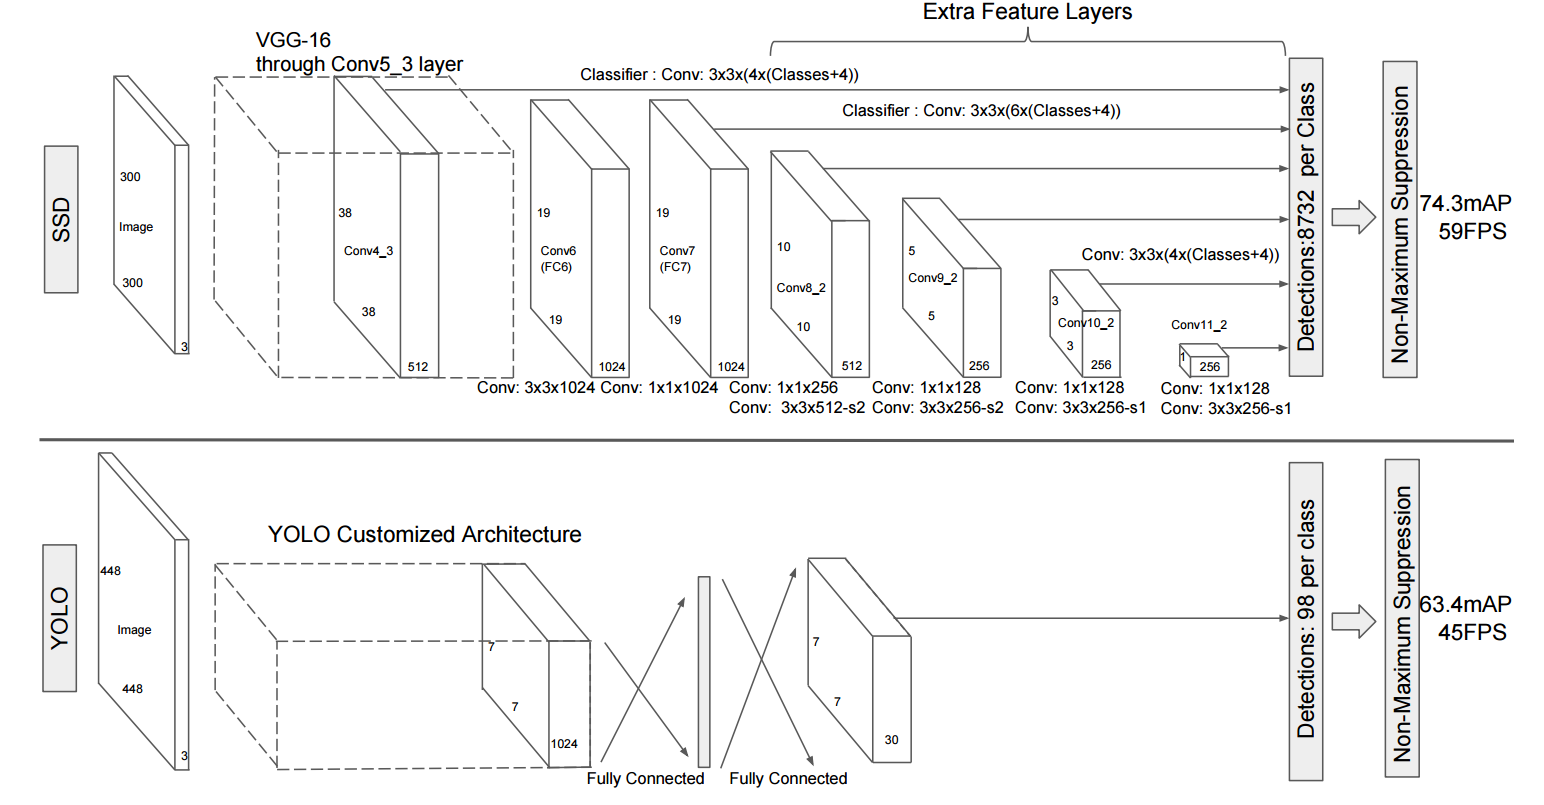
\includegraphics[width=12cm]{figures/ch2/fig6.png}
  \caption{A comparison between SSD and YOLO architectures. Adapted from \cite{liu2016ssd}.}
  \label{ch2:fig6}
\end{figure} 
 
This chapter summarised an overview of the most widely used object detectors, their novelties and their advantages along with their shortcomings. On the one hand, double-stage detectors produce region proposals and deal with detection in a later stage. On the other hand, single-stage detectors divide the images in a grid and produce boxes around each grid cell depending on a probability $p(obj)$. The trade-off between these object detector categories is that double-stage detectors usually achieve higher accuracies, while single-stage detectors are much faster.
